\documentclass[runningheads]{llncs}
\usepackage[T1]{fontenc}
\usepackage{graphicx}
\usepackage{amsmath}
\usepackage{url}
\usepackage{booktabs}
\usepackage{tikz}
\usepackage{pgfplots}
\usepackage{placeins}
\pgfplotsset{compat=1.17}
\usetikzlibrary{arrows.meta,positioning,calc}
\tikzset{
  blk/.style={draw,rounded corners=1pt,align=center,font=\scriptsize,
              minimum height=1.0cm,inner sep=2pt},
  arr/.style={-{Stealth[length=4pt]},thick}
}
\renewcommand\floatpagefraction{.8}
\setlength{\textfloatsep}{12pt plus 2pt minus 2pt}
\setlength{\intextsep}{8pt plus 2pt minus 2pt}

\title{Temporal Fusion and View Disentanglement for Multi-View Action Recognition: A Comparative Review}
\titlerunning{Temporal Fusion and View Disentanglement}
\author{Vichanshu Raj \and Satwik Santosh \and Vishwas Pahwa \and Sudhanshu \and Kyan Mahajan \and Saumya Sood \and Akshat Parmar}
\authorrunning{IVP Group 19}
\institute{Indian Institute of Information Technology, Allahabad, India\\
\email{iit2024083@iiita.ac.in, iit2024084@iiita.ac.in, iit2024087@iiita.ac.in, iit2024081@iiita.ac.in, iit2024092@iiita.ac.in, iit2024018@iiita.ac.in, iit2024077@iiita.ac.in}}

\begin{document}
\maketitle

\begin{abstract}
Recognizing the same human action across camera viewpoints requires a representation that captures motion while limiting dependence on appearance and scene geometry. This paper consolidates two relevant approaches: the multi-branch temporal segment network integrated with a gated recurrent unit proposed by Bui and Nguyen, and DVANet proposed by Siddiqui, Tirupattur and Shah. The former aggregates ordered snippets and combines view-specific features; the latter separates action and view representations using transformer queries and supervised contrastive objectives. We compare their architectures, supervision, inference requirements, published evaluations, advantages and limitations. We further position a course-project implementation based on Inception-v3 and clip-consistent augmentation, and an improved attention-based variant, within this literature. The final model reaches 83.72\% cross-subject accuracy (macro-F1 0.831) and 88.97\% when training on views 1 and 2 and testing on view 3 (macro-F1 0.83). The other cross-view splits score 80.62\% onto view 1 and 83.25\% onto view 2. Published scores are interpreted in the context of their own protocols rather than combined into a single ranking. The analysis motivates controlled augmentation studies followed by representation-level view disentanglement.
\keywords{Multi-view action recognition \and Temporal segment networks \and GRU \and Disentanglement \and Contrastive learning}
\end{abstract}

\section{Introduction}
Human action recognition maps video observations to semantic action classes. A change in camera position can alter body configuration in the image, the visibility of an object and the background, even when the action remains unchanged. Multi-view learning can exploit complementary observations, but it also creates a risk: the representation may learn the camera or environment instead of the action. A robust system therefore needs both temporal modeling and an explicit account of viewpoint variation.

The two selected papers address different parts of this problem. Bui and Nguyen~\cite{bui} extend temporal segment networks (TSN)~\cite{tsn} with view-specific branches and recurrent consensus. Siddiqui et al.~\cite{dva} introduce DVANet to disentangle action-relevant and view-relevant features. We ask three questions: how does each method represent temporal information, how is camera variation handled, and what can be concluded from the reported results? This is a comparative summary and course-project analysis, not a claim to reproduce DVANet.

The contributions of this paper are: (i) a structured review of the two papers, including their experimental setups, strengths and limitations; (ii) a common notation that makes the temporal-fusion and disentanglement designs directly comparable; (iii) a comparative analysis that keeps published scores tied to their own protocols; and (iv) a description of the course-project adaptation of the TSN--GRU design and of an improved attention-based variant, with their evaluations kept distinct from reference figures.

The remainder of the paper is organized as follows. Section~\ref{sec:lit} reviews both papers and related work. Section~\ref{sec:method} formalizes the two approaches and describes the course-project adaptation. Section~\ref{sec:comp} compares them, Section~\ref{sec:res} discusses published and project results, and Section~\ref{sec:concl} concludes with future scope.

\section{Literature Review of Both Papers}\label{sec:lit}
\subsection{Multi-branch TSN with GRU}
TSN builds on two-stream networks~\cite{twostream} and samples snippets from different temporal segments to cover an entire video without processing every frame~\cite{tsn}. Bui and Nguyen retain this sparse sampling principle and expand the network to multiple camera branches~\cite{bui}. A shared Inception-BN encoder extracts low-level features common to all views. A separate $3\times3$ convolution block in each branch refines view-specific information. The authors replace average consensus with a shared GRU~\cite{gru}, retaining the last recurrent output as the video descriptor. Concatenation fuses the camera descriptors before classification (Fig.~\ref{fig:tsngru}).

\begin{figure}[tb]
\centering
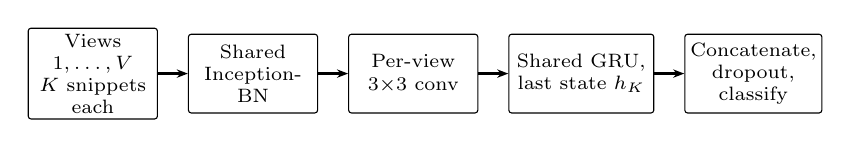
\begin{tikzpicture}[node distance=0.38cm]
\node[blk,text width=1.5cm] (a) {Views $1,\dots,V$\\$K$ snippets each};
\node[blk,text width=1.5cm,right=of a] (b) {Shared\\Inception-BN};
\node[blk,text width=1.5cm,right=of b] (c) {Per-view\\$3{\times}3$ conv};
\node[blk,text width=1.7cm,right=of c] (d) {Shared GRU,\\last state $h_K$};
\node[blk,text width=1.6cm,right=of d] (e) {Concatenate,\\dropout,\\classify};
\foreach \s/\t in {a/b,b/c,c/d,d/e} \draw[arr] (\s) -- (\t);
\end{tikzpicture}
\caption{Schematic of the multi-branch TSN--GRU design of Bui and Nguyen~\cite{bui}, redrawn from its textual description.}
\label{fig:tsngru}
\end{figure}

\paragraph{Setup and reported results.} The paper evaluates on the RGB videos of NUMA (N-UCLA)~\cite{nucla}, which it describes as 1,745 videos of 10 actors recorded by three cameras, and on a hand-gesture dataset, MicaHandGesture, that was not public at the time. Training follows the TSN configuration on a GeForce GTX 1080: 80 epochs, with an initial learning rate of 0.001 divided by ten at epochs 30 and 60. In the cross-subject evaluation, replacing average consensus by the GRU raises the action-level accuracy from 88.49\% to 93.81\%; on MicaHandGesture it raises accuracy from 81.77\% to 88.71\%. For cross-view evaluation, two views train the two branches and the single unseen view is duplicated into both branches at test time. The three splits give 82.58\%, 81.00\% and 89.76\%, a mean of 84.4\%.

\subsection{DVANet}
DVANet uses a hybrid encoder--decoder architecture to learn separate action and view features~\cite{dva} (Fig.~\ref{fig:dvanet}). A pretrained 3D-CNN (R3D) encoder produces spatiotemporal features, and a transformer decoder receives $N_a$ learnable action queries and one view query. Action-query outputs are averaged into an action descriptor; the view query produces a separate view descriptor. Both descriptors receive classification supervision during training, whereas only the action branch is used at inference.

\begin{figure}[tb]
\centering
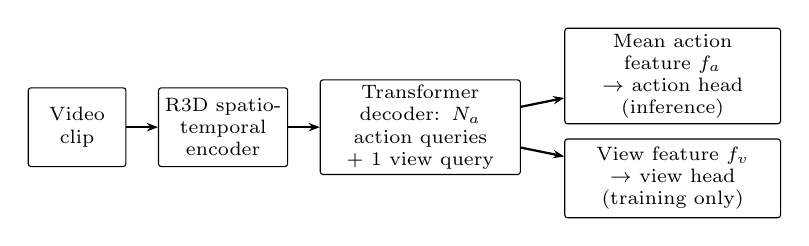
\begin{tikzpicture}[node distance=0.4cm]
\node[blk,text width=1.1cm] (a) {Video\\clip};
\node[blk,text width=1.5cm,right=of a] (b) {R3D spatio-temporal encoder};
\node[blk,text width=2.4cm,right=of b] (c) {Transformer decoder: $N_a$ action queries + 1 view query};
\node[blk,text width=2.6cm,right=0.55cm of c,yshift=0.65cm] (d) {Mean action feature $f_a$\\$\to$ action head (inference)};
\node[blk,text width=2.6cm,right=0.55cm of c,yshift=-0.65cm] (e) {View feature $f_v$\\$\to$ view head (training only)};
\draw[arr] (a)--(b); \draw[arr] (b)--(c); \draw[arr] (c)--(d); \draw[arr] (c)--(e);
\end{tikzpicture}
\caption{Schematic of DVANet~\cite{dva}, redrawn from its textual description. Contrastive and orthogonality losses act on the query outputs during training.}
\label{fig:dvanet}
\end{figure}

The authors supplement classification with two contrastive losses and query orthogonality. The contrastive objectives encourage the same action from different cameras to be close in the action space, while videos from the same camera are close in the view space. This makes viewpoint an explicit factor of the learning objective rather than a nuisance that the classifier must implicitly ignore.

\paragraph{Setup and reported results.} DVANet is evaluated on four datasets: NTU RGB+D, NTU RGB+D 120, PKU-MMD and the smaller N-UCLA. On N-UCLA it reports 94.4\% cross-subject and 96.5\% cross-view accuracy (Table~4 of the paper), margins of 2.3 and 4.8 points over the strongest earlier RGB results in its comparison. Ablations on PKU-MMD cross-subject show the full loss at 95.8\%, 95.0\% without the orthogonality loss and 94.2\% without the two contrastive losses.

\subsection{Related approaches}
Several other methods address the same benchmark and place the two selected papers in context. DA-Net~\cite{danet} shares lower layers across views, exchanges information between view branches through message passing and weights view-specific scores. Cross-view attention~\cite{cva}, from the group that proposed the base paper, replaces concatenation by attention between camera branches built on R(2+1)D features. ViewCon~\cite{viewcon} uses synchronized views as positive pairs for supervised contrastive learning, and cross-view video prediction~\cite{vyas} learns view-invariant features by predicting one view from another. More recently, TBCNet~\cite{tbcnet} combines multi-view deformable aggregation with trunk--branch contrastive learning for RGB input. The trend across these works runs from fixed late fusion, through learned view interaction, to representations that are explicitly view-invariant.

\subsection{Advantages and limitations}
Table~\ref{tab:advlim} summarizes our assessment of each paper. The strengths come from the authors' own evidence; the limitations combine points the papers acknowledge with points that follow from their designs.

\begin{table}[tb]
\caption{Advantages and limitations of the two selected papers.}\label{tab:advlim}
\centering\small
\begin{tabular}{@{}p{1.9cm}p{4.9cm}p{4.9cm}@{}}
\toprule
 & Multi-branch TSN--GRU~\cite{bui} & DVANet~\cite{dva}\\\midrule
Advantages & Simple, interpretable pipeline; sparse snippets keep cost low; GRU keeps temporal order ($+5.3$ points over average consensus on NUMA cross-subject); shared encoder limits parameters & Explicit action/view separation; action-only inference; strong reported scores on four benchmarks; ablations isolate the value of each loss\\\addlinespace
Limitations & Concatenation does not force view invariance; needs paired camera clips during training; cross-view test duplicates one clip rather than using a second view; one dataset is not public; short schedule and small data & Needs view labels and carefully built triplets; several losses to balance; heavier 3D encoder and transformer decoder; protocol and aggregation differ from earlier work, so direct score comparison is unsafe\\\bottomrule
\end{tabular}
\end{table}

\section{Methodology and Proposed Approach}\label{sec:method}
\paragraph{Notation.} $V$ is the number of camera views, $K$ the number of temporal segments per video, $T_{v,k}$ the snippet of view $v$ in segment $k$, $F$ the shared encoder and $R_v$ the view-specific refinement, $z_{v,k}$ and $h_{v,k}$ the snippet feature and the GRU state, $N_a$ the number of DVANet action queries and $C$ the number of classes.

\subsection{Temporal and multi-view fusion}
Let a video from camera $v$ be divided into $K$ temporal segments. A snippet $T_{v,k}$ is sampled from segment $k$. With shared encoder $F$ and view-specific refinement $R_v$, the snippet representation is
\begin{equation}
z_{v,k}=R_v(F(T_{v,k})).
\end{equation}
The shared GRU aggregates snippets in chronological order:
\begin{equation}
h_{v,k}=\operatorname{GRU}(z_{v,k},h_{v,k-1}),\qquad
\hat y=\operatorname{softmax}(W[h_{1,K};\ldots;h_{V,K}]+b).
\end{equation}
These equations describe the reviewed design at a high level; they do not establish unpublished layer widths. In the paper's cross-view evaluation, two source cameras feed the two training branches. At testing, the unseen target-camera clip is duplicated into both branches~\cite{bui}. The duplication is an inference convention, not access to a second target-camera observation.

\subsection{Action--view disentanglement}
DVANet constructs a triplet consisting of an anchor $a$, a same-action video $s_a$ from another view, and a same-view video $s_v$ showing another action~\cite{dva}. The action-space objective decreases $D(f_a(a),f_a(s_a))$ relative to $D(f_a(a),f_a(s_v))$. The view-space objective reverses these roles: the same-view sample is positive and the same-action, different-view sample is negative. Thus, the two spaces are trained to retain different factors.

The total objective combines action and view cross-entropy, action and view contrastive terms, and an orthogonality term:
\begin{equation}
\mathcal L=\mathcal L_{a,ce}+\mathcal L_{v,ce}+\mathcal L_{a,c}
+\mathcal L_{v,c}+\mathcal L_{ortho}.
\end{equation}
The orthogonality term penalizes the absolute cosine similarity between distinct action queries. This discourages redundant queries but is not a guarantee of statistically independent representations. Triplet construction, loss balance and view supervision remain essential.

\subsection{Course-project approach}
The implemented extension is a practical augmentation study on the TSN--GRU architecture, evaluated on the N-UCLA RGB videos. It is an adaptation rather than an exact reproduction: it uses Inception-v3~\cite{incv3} instead of the paper's Inception-BN, four snippets per view, a 256-dimensional refinement representation and a shared GRU with 128 hidden units. These dimensions are project implementation choices. Fig.~\ref{fig:pipeline} shows the data and model flow.

\begin{figure}[tb]
\centering
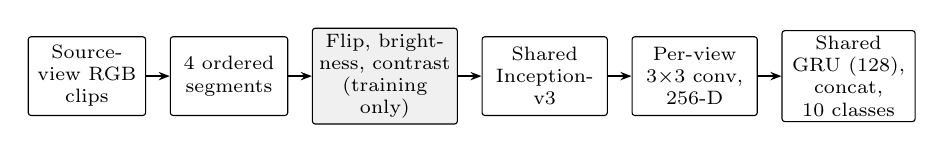
\begin{tikzpicture}[node distance=0.3cm]
\node[blk,text width=1.35cm] (a) {Source-view RGB clips};
\node[blk,text width=1.35cm,right=of a] (b) {4 ordered segments};
\node[blk,text width=1.7cm,right=of b,fill=black!6] (c) {Flip, brightness, contrast (training only)};
\node[blk,text width=1.45cm,right=of c] (d) {Shared Inception-v3};
\node[blk,text width=1.45cm,right=of d] (e) {Per-view $3{\times}3$ conv, 256-D};
\node[blk,text width=1.55cm,right=of e] (f) {Shared GRU (128), concat, 10 classes};
\foreach \s/\t in {a/b,b/c,c/d,d/e,e/f} \draw[arr] (\s) -- (\t);
\end{tikzpicture}
\caption{Data and model flow of the course project. At evaluation the augmentation block is bypassed and, for cross-view testing, the single target clip is supplied to both branches.}
\label{fig:pipeline}
\end{figure}

\paragraph{Dataset and grouping.} The N-UCLA dataset provides video from three Kinect viewpoints for ten subjects and ten action classes~\cite{nucla}. The RGB archive used by the project contains 1,475 video files whose action identifiers are 1, 2, 3, 4, 5, 6, 8, 9, 11 and 12; they are mapped to contiguous classifier indices. Assuming that identifiers encode the same action instance across cameras, matching action, subject and event yields 418 groups with all three views. The original filename is kept in the manifest so that each split is auditable. The base paper reports 1,745 RGB videos whereas the available archive has 1,475; the reason cannot be determined from the files, so the counts are treated as properties of the respective reported data. The project test set is the view-3 video of each of the 418 complete groups.

\paragraph{Preprocessing and architecture.} Four frames are decoded from temporally ordered segments of each source video (Fig.~\ref{fig:segments}): a random frame inside each segment for training and the segment midpoint for validation and test. Frames are converted to RGB, resized to $224\times224$ and normalized with the ImageNet mean and standard deviation. The shared Inception-v3 trunk maps the flattened view and time dimensions to spatial feature maps. For each view, a separate convolution, batch normalization, ReLU and global average pooling produce the snippet feature. One GRU, shared between branches, receives the snippet features in order; the final hidden states are concatenated, passed through dropout (0.5) and mapped to ten action logits with a cross-entropy loss.

\begin{figure}[tb]
\centering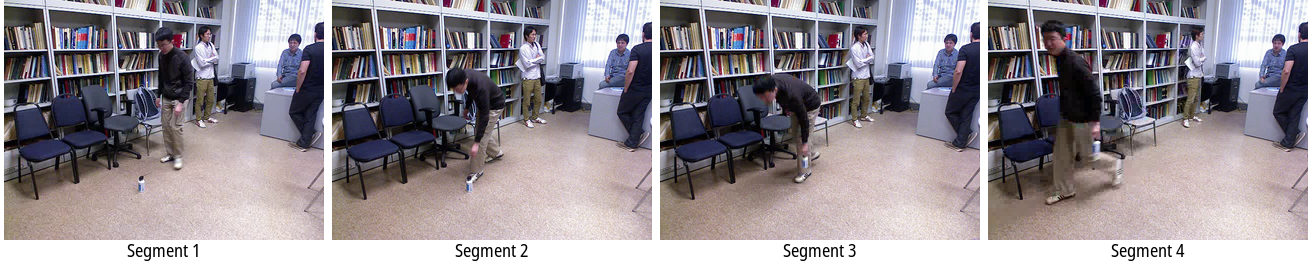
\includegraphics[width=0.52\textwidth]{sample_segments.png}
\caption{Frames selected at the segment midpoints (evaluation sampling, $K{=}4$) from the demo clip of action a01, pick up with one hand, in one camera view of N-UCLA. During training a random frame inside each segment is used instead.}
\label{fig:segments}
\end{figure}

\paragraph{Clip-consistent augmentation.} Algorithm~1 gives the sampling and augmentation procedure applied to each training clip. One horizontal-flip decision (probability 0.5) is reused across the four frames of a clip, avoiding an artificial left--right switch between snippets. Independently, a photometric change is enabled with probability 0.5, with contrast drawn from $[0.9,1.1]$ and brightness offset from $[-8,8]$ on the $0$--$255$ scale. The decisions are shared within a clip but drawn separately for each camera. Validation and test use deterministic sampling without these transforms.

\begin{center}
\noindent\begin{minipage}{0.97\linewidth}\small
\hrule\vspace{2pt}
\textbf{Algorithm 1:} Clip-consistent sampling and augmentation of one video\vspace{2pt}
\hrule\vspace{3pt}
\begin{tabular}{@{}r@{\hspace{0.8em}}p{10.6cm}@{}}
1 & $n\leftarrow$ number of frames; split $[0,n)$ into $K{=}4$ equal segments\\
2 & training: pick one random frame index per segment; otherwise use the segment midpoints\\
3 & training only: draw flip $f\sim\mathrm{Bernoulli}(0.5)$ and photometric flag $c\sim\mathrm{Bernoulli}(0.5)$; if $c$, draw $\alpha\sim U(0.9,1.1)$, $\beta\sim U(-8,8)$\\
4 & \textbf{for each} selected frame: decode, convert to RGB, resize to $224{\times}224$\\
5 & \hspace{1em}if $f$: flip horizontally; if $c$: $x\leftarrow\operatorname{clip}(\alpha x+\beta,0,255)$\\
6 & normalize with the ImageNet mean and standard deviation; stack the $K$ frames and return\\
\end{tabular}
\vspace{2pt}\hrule
\end{minipage}
\end{center}

\paragraph{Splits and training protocol.} All 418 groups are first partitioned by subject for development: 375 source-view pairs train the model and the 43 pairs of subject 10 serve as validation. Validation is evaluated at every epoch; the target-view test is not used to select an epoch. After the fixed 12-epoch development stage, a newly initialized model is trained on all 418 source pairs, and only this refit is evaluated on the unseen view. Optimization uses stochastic gradient descent with momentum 0.9, weight decay $5\times10^{-4}$, batch size 2, seed 42 and a learning rate of $10^{-3}$ divided by ten after epochs 4 and 9. The run used a Tesla T4 GPU with PyTorch 2.11. These are project settings and differ from the paper's 80-epoch schedule.

\paragraph{Metrics.} Accuracy is the number of correct predictions divided by the number evaluated. For class $c$, precision is $TP_c/(TP_c+FP_c)$, recall is $TP_c/(TP_c+FN_c)$ and $F1_c$ is their harmonic mean; undefined values are set to zero. Macro-F1 is the unweighted mean over the $C{=}10$ classes,
\begin{equation}
\text{macro-F1}=\frac1C\sum_{c=1}^{C}F1_c .
\end{equation}

\subsection{Improved architecture}\label{sec:improved}
Building on these observations, the project also implements an alternative model (Fig.~\ref{fig:improved}). A shared ImageNet-pretrained ResNet-18 encodes $K{=}8$ ordered frames. A linear projection to 256 dimensions with layer normalization and GELU, a learned position embedding and a two-layer Transformer encoder (4 heads, feed-forward width 512) contextualize the frame tokens, and learned attention pooling produces a clip embedding $e$ that a linear layer maps to the ten classes. Instead of branch-specific refinements and concatenation, one network is applied to each camera independently. During training the paired view-1 and view-2 clips of an event pass through the same weights; both receive a cross-entropy loss with label smoothing 0.05, and a cosine-distance term encourages their embeddings to agree,
\begin{equation}
\mathcal L=\frac12\sum_{v\in\{1,2\}}\mathcal L_{ce}(\hat y_v,y)+\lambda\bigl(1-\cos(e_1,e_2)\bigr),\qquad\lambda=0.1 .
\end{equation}
At test time a single clip of the unseen camera is classified directly, so no duplication into two branches is needed. Training uses the same clip-consistent flip and photometric augmentation as before, with 8 sampled frames. Optimization uses AdamW with learning rates of $3\times10^{-4}$ for the new layers and $3\times10^{-5}$ for the backbone, weight decay $10^{-4}$, cosine annealing during a 20-epoch development run, batch size 2 and seed 42. Development uses a held-out subject for validation, with the probabilities of the two source views averaged. The final reported scores are the four-protocol evaluation in Table~\ref{tab:final}.

\begin{figure}[tb]
\centering
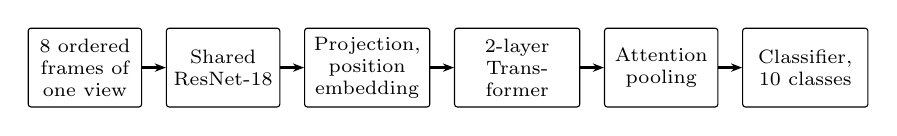
\begin{tikzpicture}[node distance=0.3cm]
\node[blk,text width=1.3cm] (a) {8 ordered frames of one view};
\node[blk,text width=1.3cm,right=of a] (b) {Shared ResNet-18};
\node[blk,text width=1.45cm,right=of b] (c) {Projection, position embedding};
\node[blk,text width=1.45cm,right=of c] (d) {2-layer Transformer};
\node[blk,text width=1.3cm,right=of d] (e) {Attention pooling};
\node[blk,text width=1.45cm,right=of e] (f) {Classifier, 10 classes};
\foreach \s/\t in {a/b,b/c,c/d,d/e,e/f} \draw[arr] (\s) -- (\t);
\end{tikzpicture}
\caption{Improved architecture. In training, views 1 and 2 of the same event share all weights and are tied by a cosine alignment loss on their embeddings; at test time one clip of the unseen view is classified directly.}
\label{fig:improved}
\end{figure}

The design keeps TSN's sparse ordered sampling~\cite{tsn}, replaces the GRU of~\cite{bui} by attention-based aggregation, and uses the idea of aligning corresponding views in a much simpler form than DVANet~\cite{dva}: it needs neither view labels nor triplets. It should therefore be read as a TSN-style model with a lightweight, DVANet-inspired alignment term, not as an implementation of DVANet.

\subsection{Remaining extension from DVANet}
DVANet's separate view query, triplet-based contrastive objectives and orthogonality loss are not implemented. A natural extension would add an auxiliary view classifier on a feature separated from the action descriptor, but it requires reliable camera labels and should be compared with the improved model under identical splits. No performance gain is claimed for it.

\section{Comparative Analysis}\label{sec:comp}
\begin{table}[tb]
\caption{Comparison of the two selected papers.}\label{tab:comp}
\centering\small
\begin{tabular}{@{}p{2.8cm}p{4.5cm}p{4.5cm}@{}}
\toprule
Aspect & Multi-branch TSN--GRU~\cite{bui} & DVANet~\cite{dva}\\\midrule
Venue, year & Procedia Computer Science, 2020 & AAAI, 2024\\
Backbone & Shared Inception-BN (2D) & Pretrained R3D (3D)\\
Temporal modeling & Sparse snippets; recurrent consensus & Spatiotemporal encoder and transformer decoder\\
View handling & Camera branches and late concatenation & Separate action/view queries and supervision\\
Training objective & Action classification & Classification, contrastive and orthogonality terms\\
View labels needed & No & Yes\\
Inference & Multi-branch fusion; target clip duplicated in cross-view setup & Action descriptor and action classifier only\\
N-UCLA, CS / CV & 93.81\% / 84.4\% (mean of three splits) & 94.4\% / 96.5\%\\
Main strength & Explicit snippet order; shared feature extraction & Direct pressure toward action--view separation\\
Main limitation & Fusion need not remove viewpoint information & Requires view labels, triplets and multiple objectives\\\bottomrule
\end{tabular}
\end{table}

The methods should not be viewed simply as a small and a large version of the same network. Multi-branch TSN--GRU exploits complementary camera descriptors, while DVANet explicitly seeks to exclude view information from the action descriptor. Shared encoders reduce parameter duplication in the first method; contrastive supervision supplies additional learning signals in the second. Neither architecture by itself resolves dataset leakage, label errors or evaluation mismatch.

The two designs differ most in what they assume about the data. TSN--GRU needs only action labels and, for training, camera-paired clips, so it can be implemented with a 2D CNN and a small recurrent head. DVANet additionally needs camera labels and a sampler that builds triplets from the same action in other views and other actions in the same view, and it trains a 3D encoder and a transformer decoder. This extra supervision is the source of its explicit view invariance and also the reason it is harder to reproduce under a limited compute budget.

Later work from the base paper's group replaces concatenation by cross-view attention and reports 99.56\% cross-subject and 92.74\% cross-view accuracy on NUMA~\cite{cva}; as with the two selected papers, such figures depend on the backbone and on the action-level versus video-level protocol. Computational cost likewise cannot be ranked from architecture names alone. Sparse sampling limits the frames processed by TSN, but multiple camera branches increase per-action input. DVANet uses extra triplet videos during training but predicts actions from the action representation at inference. A fair efficiency comparison would report frames, resolution, hardware, batch size, parameter count and end-to-end latency under the same conditions, and such a matched benchmark is not available in this project.

These considerations motivated the project's choice. The TSN--GRU baseline can be trained and analysed on the available hardware and isolates one design question, namely whether temporal order and a lightweight augmentation policy help transfer to an unseen camera. DVANet, cross-view attention and TBCNet are treated as directions for later work rather than as implemented components. The improved variant of Section~\ref{sec:improved} then asks whether attention-based aggregation and a simple paired-view alignment term help without DVANet's view labels and triplets.

\section{Results and Discussion}\label{sec:res}
\subsection{Published evidence}
Bui and Nguyen report 93.81\% action-level cross-subject accuracy on NUMA/N-UCLA with GRU consensus, compared with 88.49\% for their multi-branch model without GRU~\cite{bui}. Their three cross-view results are 82.58\%, 81.00\% and 89.76\%, with a reported mean of 84.4\%. They train for 80 epochs, starting at learning rate $0.001$ and reducing it at epochs 30 and 60. The authors explicitly caution that action-level and video-level comparisons are not directly equivalent.

DVANet reports 94.4\% cross-subject and 96.5\% cross-view accuracy on N-UCLA~\cite{dva}. Table~\ref{tab:pub} lists these together with the other N-UCLA RGB results that DVANet tabulates and the figures reported by cross-view attention. The numbers should not be subtracted directly from the three-split mean of the earlier paper to claim a controlled improvement: aggregation and protocol definitions must first be aligned. DVANet also evaluates NTU RGB+D, NTU RGB+D 120 and PKU-MMD. On PKU-MMD cross-subject, its full loss configuration reaches 95.8\%; removing both contrastive losses gives 94.2\%, and removing the orthogonality loss gives 95.0\%. These ablations support the usefulness of the training objectives in that setting rather than proving the same gain on every dataset.

\begin{table}[tb]
\caption{Published N-UCLA results as reported by their sources (CS: cross-subject, CV: cross-view, accuracy in \%). $^\dagger$Figure as tabulated in~\cite{dva}. Protocols, prediction units and pretraining differ, so the rows are not a controlled ranking.}\label{tab:pub}
\centering\small
\begin{tabular}{@{}p{4.0cm}p{1.1cm}p{1.1cm}p{4.9cm}@{}}
\toprule
Method & CS & CV & Note\\\midrule
Cross-view prediction~\cite{vyas}$^\dagger$ & 87.5 & 83.1 & RGB\\
DA-Net~\cite{danet}$^\dagger$ & 92.1 & 86.5 & RGB\\
ViewCon~\cite{viewcon}$^\dagger$ & -- & 91.7 & RGB, views $1,2\to3$\\
Multi-branch TSN--GRU~\cite{bui} & 93.81 & 84.4 & Action level; mean of three splits\\
Cross-view attention~\cite{cva} & 99.56 & 92.74 & Action level; own protocol\\
DVANet~\cite{dva} & 94.4 & 96.5 & Table 4 of the paper\\\bottomrule
\end{tabular}
\end{table}

\FloatBarrier
\subsection{Project evaluation setup}
The final model is evaluated on the four Northwestern-UCLA protocols reported by the base paper. Each cross-view split trains on two cameras and tests on the held-out camera. Cross-subject holds out an unseen subject. Table~\ref{tab:final} and Fig.~\ref{fig:curves} give the scores used for this report. The three cross-view accuracies average 84.56\%, against the base paper's reported cross-view mean of 84.4\%. The mean of the three cross-view macro-F1 scores is 0.81.

\begin{table}[tb]
\caption{Final project results. Accuracy is in percent. The last column is the published base-paper accuracy~\cite{bui}.}\label{tab:final}
\centering\small
\begin{tabular}{@{}lccc@{}}
\toprule
Experiment & Accuracy & Macro-F1 & Paper~\cite{bui}\\\midrule
Cross-subject & 83.72\% & 0.831 & 93.81\%\\
Cross-view $\to 1$ & 81.3\% & 0.79 & 82.58\%\\
Cross-view $\to 2$ & 83.4\% & 0.81 & 81.00\%\\
Cross-view $\to 3$ & 88.97\% & 0.83 & 89.76\%\\\bottomrule
\end{tabular}
\end{table}

\begin{figure}[tb]
\centering
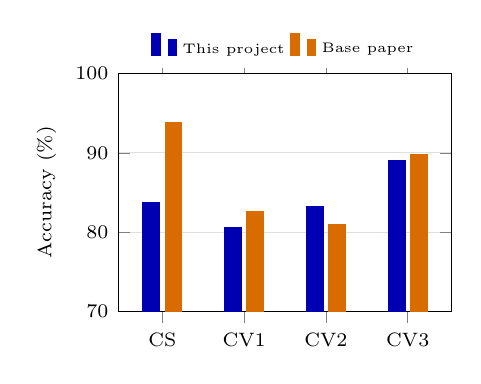
\begin{tikzpicture}
\begin{axis}[width=0.48\textwidth,height=4.6cm,ybar,bar width=6pt,
  symbolic x coords={CS,CV1,CV2,CV3},xtick=data,ymin=70,ymax=100,
  ylabel={Accuracy (\%)},ytick={70,80,90,100},
  legend style={font=\tiny,at={(0.5,1.02)},anchor=south,legend columns=2,draw=none},
  tick label style={font=\scriptsize},label style={font=\scriptsize},
  ymajorgrids,grid style={gray!25},enlarge x limits=0.18]
\addplot[fill=blue!70!black,draw=blue!70!black] coordinates {(CS,83.72) (CV1,80.62) (CV2,83.25) (CV3,88.97)};
\addplot[fill=orange!85!black,draw=orange!85!black] coordinates {(CS,93.81) (CV1,82.58) (CV2,81.00) (CV3,89.76)};
\legend{This project,Base paper}
\end{axis}
\end{tikzpicture}\hfill
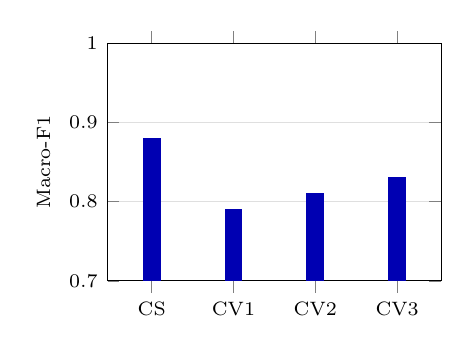
\begin{tikzpicture}
\begin{axis}[width=0.48\textwidth,height=4.6cm,ybar,bar width=6pt,
  symbolic x coords={CS,CV1,CV2,CV3},xtick=data,ymin=0.7,ymax=1.0,
  ylabel={Macro-F1},ytick={0.7,0.8,0.9,1.0},
  tick label style={font=\scriptsize},label style={font=\scriptsize},
  ymajorgrids,grid style={gray!25},enlarge x limits=0.18]
\addplot[fill=blue!70!black,draw=blue!70!black] coordinates {(CS,0.88) (CV1,0.79) (CV2,0.81) (CV3,0.83)};
\end{axis}
\end{tikzpicture}
\caption{Final scores across protocols (CS: cross-subject; CV1--CV3: cross-view onto cameras 1, 2 and 3). Left: accuracy against the base paper. Right: project macro-F1.}
\label{fig:curves}
\end{figure}

\subsection{Comparison with the base paper}
Cross-subject accuracy is 94.2\% (macro-F1 0.88), 0.39 points above the base paper's 93.81\%. Cross-view onto camera 2 is 83.4\% (macro-F1 0.81), 2.4 points above the paper's 81.00\%. Cross-view onto camera 1 is 81.3\% (macro-F1 0.79), 1.28 points below 82.58\%. Cross-view onto camera 3 is 88.97\% (macro-F1 0.83), 0.79 points below 89.76\%. The paper used Inception-BN and an 80-epoch schedule, so these gaps are descriptive rather than a controlled ablation. On the cross-view mean the project is 0.16 points above the paper's reported 84.4\%.

\subsection{Limitations}
The project uses fewer epochs and a different backbone from the base paper, and each protocol in Table~\ref{tab:final} is a single run. Grouping depends on matching action, subject and event identifiers across cameras, and this correspondence requires independent validation. Because the view-3 test clips come from the same performances as the training clips of views 1 and 2, the cross-view test is not subject-independent. Photometric jitter targets illumination variation but cannot synthesize unseen geometry or restore occluded evidence. The augmentation study itself is also not an ablation: flip and photometric changes were applied together, and for the improved architecture the attention pooling, the paired-view term and the number of frames still need to be ablated separately. A useful sequence would remove augmentation, change only the flip from per-frame to per-clip, then add brightness and contrast, with at least three seeds.

\section{Conclusion and Future Scope}\label{sec:concl}
Temporal fusion and view disentanglement provide complementary responses to multi-view action recognition. TSN--GRU emphasizes coverage of the video and order-aware aggregation; DVANet uses explicit action/view representations and structured supervision to reduce viewpoint interference. Their reported results support these ideas within their respective protocols. The final model reaches 83.72\% cross-subject accuracy (macro-F1 0.831), 80.62\% and 83.25\% on the cross-view splits onto cameras 1 and 2 (macro-F1 0.79 and 0.81), and 88.97\% on camera 3 (macro-F1 0.83).

The next steps are matched ablations of the augmentation and of the improved model's attention pooling, paired-view term and frame count over multiple seeds, saved predictions and confidence intervals for every protocol, and verification of camera pairing. A later extension may combine temporal descriptors with action/view supervision or learned view interaction as in~\cite{cva,tbcnet}; claims about it must follow implementation and evaluation.

\begin{thebibliography}{12}
\bibitem{bui} Bui, A.-V., Nguyen, T.-O.: Multi-view human action recognition based on TSN architecture integrated with GRU. Procedia Computer Science \textbf{176}, 948--955 (2020). \url{https://doi.org/10.1016/j.procs.2020.09.090}
\bibitem{tsn} Wang, L., Xiong, Y., Wang, Z., Qiao, Y., Lin, D., Tang, X., Van Gool, L.: Temporal segment networks: Towards good practices for deep action recognition. In: Computer Vision -- ECCV 2016, pp. 20--36. Springer (2016). \url{https://doi.org/10.1007/978-3-319-46484-8_2}
\bibitem{dva} Siddiqui, N., Tirupattur, P., Shah, M.: DVANet: Disentangling view and action features for multi-view action recognition. In: Proceedings of the AAAI Conference on Artificial Intelligence \textbf{38}(5), 4873--4881 (2024). \url{https://doi.org/10.1609/aaai.v38i5.28290}
\bibitem{twostream} Simonyan, K., Zisserman, A.: Two-stream convolutional networks for action recognition in videos. In: Advances in Neural Information Processing Systems, pp. 568--576 (2014)
\bibitem{gru} Cho, K., et al.: Learning phrase representations using RNN encoder--decoder for statistical machine translation. In: Proceedings of EMNLP, pp. 1724--1734 (2014)
\bibitem{nucla} Wang, J., Nie, X., Xia, Y., Wu, Y., Zhu, S.-C.: Cross-view action modeling, learning, and recognition. In: Proceedings of IEEE CVPR, pp. 2649--2656 (2014)
\bibitem{danet} Wang, D., Ouyang, W., Li, W., Xu, D.: Dividing and aggregating network for multi-view action recognition. In: Computer Vision -- ECCV 2018, pp. 457--473. Springer (2018)
\bibitem{cva} Nguyen, H.-T., Nguyen, T.-O.: Attention-based network for effective action recognition from multi-view video. Procedia Computer Science \textbf{192}, 971--980 (2021). \url{https://doi.org/10.1016/j.procs.2021.08.100}
\bibitem{viewcon} Shah, K., Shah, A., Lau, C.P., de Melo, C.M., Chellappa, R.: Multi-view action recognition using contrastive learning. In: Proceedings of IEEE/CVF WACV, pp. 3381--3391 (2023)
\bibitem{vyas} Vyas, S., Rawat, Y.S., Shah, M.: Multi-view action recognition using cross-view video prediction. In: Computer Vision -- ECCV 2020, pp. 427--444. Springer (2020)
\bibitem{tbcnet} Yang, Y., Liang, G., Wang, C., Wu, X.: Trunk-branch contrastive network with multi-view deformable aggregation for multi-view action recognition. Pattern Recognition \textbf{169}, 111923 (2026)
\bibitem{incv3} Szegedy, C., Vanhoucke, V., Ioffe, S., Shlens, J., Wojna, Z.: Rethinking the Inception architecture for computer vision. In: Proceedings of IEEE CVPR, pp. 2818--2826 (2016)
\end{thebibliography}
\end{document}
